% ECTEL 2026 - Full Research Paper
% paper2.tex -- revised version
%
\documentclass[runningheads]{llncs}
%
\usepackage[T1]{fontenc}
\usepackage{graphicx}
\usepackage{amsmath, amsfonts, amssymb}
\usepackage{tabularx}
\usepackage{booktabs}
\usepackage{hyperref}
\usepackage[markup=underlined, authormarkup=none]{changes}
\usepackage{subcaption}
\usepackage{float}
\definechangesauthor[name=Development, color=blue]{dev}
%
\graphicspath{{img/}}
%
\begin{document}
%
\title{Grounding User Models in Learning Theory for Actionable Strategies}
%
\titlerunning{Grounding User Models in Learning Theory for Actionable Strategies}
\author{Anonymous}
\authorrunning{Anonymous}
\institute{Anonymous Institution}
%
\maketitle
%
\begin{abstract}

Intelligent Tutoring Systems (ITS) rely on student models to drive adaptive instruction, yet the Knowledge Tracing approaches that underpin these models have been developed almost exclusively to optimise predictive accuracy. The resulting representations are either interpretable but rigid, as in classical Bayesian Knowledge Tracing (BKT), or accurate but opaque, as in deep knowledge tracing approaches. Neither type produces actionable outputs that educators can inspect, validate, or act upon directly. While recent work has proposed \textit{representational grounding} as a design principle for interpretable deep knowledge tracing, it has not addressed how the resulting theory-grounded parameters can be integrated into an ITS in order to support purposeful instructional decisions. The present paper addresses this gap by presenting the design of an \textit{augmented student model} that translates the outputs of such grounded knowledge tracing models into instructionally actionable representations. Specifically, we show how continuously updated estimates of prior knowledge and learning rate can be used to assign each student to one of the \textit{learning situations} defined by a data-driven partition of the parameter space, and how each situation implies a distinct and evidence-grounded instructional strategy. The result is a student-centred design in which pedagogically-grounded instructional strategies are continuously adapted to learners' evolving needs, with transparency and educator agency as first-class concerns.

\keywords{deep knowledge tracing \and intelligent tutoring systems \and user modeling \and grounded transformers \and representational grounding}
\end{abstract}
%
%
\section{Introduction}

Intelligent Tutoring Systems (ITS) \cite{itssleeman82} rely on user models that capture the learner's evolving state of mastery and supply the evidence from which instructional strategies are derived. In most deployed systems, mastery states are inferred using Knowledge Tracing (KT) approaches, ranging from Bayesian Knowledge Tracing (BKT)~\cite{corbett1994knowledge} to deep knowledge tracing architectures that evolved from early recurrent neural network models such as DKT~\cite{piech2015deep} to more recent attention-based Transformer architectures~\cite{ghosh2020context}. While deep learning has significantly advanced the predictive accuracy of KT, the field has become increasingly detached from the learning theories and pedagogical principles that should guide instruction. This orientation towards accuracy-driven opacity creates a fundamental design gap in the development of ITS, which require learner representations that are not only accurate but also mindful of pedagogical intent. Specifically, while recent work on \textit{representational grounding} has shown that Transformer architectures can be anchored to theory-based constructs~\cite{labra2026theory}, there remains a need to demonstrate how such theory-rooted parameters can be operationalised into purposeful user models that support transparent and accountable instructional practice.

The present paper addresses this gap by adopting the principles of transparency and pedagogical purpose as primary design requirements for user modeling. Drawing on the theory-grounded parameters provided by grounded Transformers, we present the design of an \textit{augmented user model} that transforms longitudinal learning signals into pedagogically recognisable \textit{learning situations}. Our contribution is twofold: first, we demonstrate how theory-rooted parameter estimates can be used to construct an augmented user model capable of supporting situation-based diagnostics; and second, we show how these learning situations support differentiated instructional strategies that adapt dynamically to each student's evolution. This mindful approach ensures that technological innovation remains anchored in pedagogical purpose, empowering educators with the agency necessary to make sensible, evidence-grounded decisions while providing the transparency and accountability required in high-stakes educational environments.

The research question that guides this work is: 

\textit{RQ: How can ITS user modeling be augmented with theory-grounded information to support more mindful instructional strategies that comply with the requirements for transparency and pedagogical purpose?}

The remainder of the paper is organised as follows. Section~2 provides background on the learning theories and the gTransformer architecture. Section~3 establishes the design principles of the augmented user model. Section~4 describes the methodology for operationalising this model. Section~5 presents the empirical results and discussion. Section~6 concludes.

%

\section{Background}

In this section, we first introduce BKT as the theoretical anchor providing the semantic parameters required for pedagogical grounding. We then describe gTransformer as the deep learning architecture that transforms population-level parameters from reference models such as BKT into student-specific parameters by encoding context from individual interaction histories. Finally, we review the core components of an ITS, framing the user and tutorial models as mediators of pedagogical intent that support the translation of learner activity into purposeful instructional action.

\subsection{Learning Theories and Bayesian Knowledge Tracing}

We select BKT~\cite{corbett1994knowledge} as our reference theoretical framework. BKT models the learning process as a Hidden Markov process governed by four interpretable parameters:

\begin{itemize}
    \item \textit{Initial Mastery} ($P(\text{L}_0)$): the probability that a student knows a concept prior to practice.
    \item \textit{Learn Rate} ($P(\text{T})$): the probability of transitioning from the unlearned to the learned state.
    \item \textit{Guess} ($P(\text{G})$): the probability of a correct response despite lack of mastery.
    \item \textit{Slip} ($P(\text{S})$): the probability of an incorrect response despite mastery.
\end{itemize}

These parameters provide the \textit{theoretical anchor} required for transparency, enabling a recursive estimation of student mastery that corresponds to recognisable learning constructs.

However, traditional BKT is limited by its population-level assumptions: it typically estimates a single parameter set for all students on a given skill~\cite{yudelson2013individualized}. As a result, learners with identical recent response patterns receive the same mastery estimate regardless of their individual learning history. To support mindful, personalised instruction, these theoretical constructs must be made longitudinally sensitive and reflective of individual learning dynamics. The augmented student model proposed here addresses this by leveraging gTransformer to derive student-specific parameters from population-level BKT estimates.

\subsection{Deep Knowledge Tracing and Grounded Transformers}

Historically, KT has been characterized by a dichotomy between two paradigms: traditional models like BKT~\cite{corbett1994knowledge}, which are \textit{intrinsically interpretable} due to their human-understandable parameters, and deep learning architectures introduced in DKT~\cite{piech2015deep} that have demonstrated superior predictive accuracy but operate as opaque ``black boxes'' whose internal states lack direct correspondence to pedagogical principles~\cite{abdelrahman2023knowledge}. This lack of transparency raises significant concerns regarding accountability in high-stakes educational environments~\cite{rudin2019stop}. Grounded Transformers such as gTransformer~\cite{labra2026theory} emerge as an alternative to this dichotomy, proposing an architecture that maintains the predictive power of deep learning while ensuring its internal representations are grounded in established learning theories~\cite{labra2026theory}.

The gTransformer architecture, shown in Fig.~\ref{fig_overview}, is designed to transform learner activity history into actionable pedagogical information through three distinct stages:

\begin{itemize}
  \item Input: The model integrates raw interaction histories with theoretical priors derived from population-level BKT estimates. This anchoring ensures that the architecture remains grounded in pedagogically sound principles.
  \item Processing: Within the core engine, two parallel tracks process the student's context. The \textit{standard track} optimizes for estimations accuracy, while the \textit{grounded track} projects latent context onto theory-defined axes to derive student-specific parameters ($p_{\text{L}_0}, p_{\text{T}}$). Both tracks are jointly optimized via a multi-objective loss that enforces both inference accuracy and grounding.
  \item Output: The resulting grounded parameters quantify each learner's unique dynamics. They form the data-driven basis of the augmented user model.
\end{itemize}

\begin{figure}[!htb]
\centering

\includegraphics[width=\textwidth]{arch2.png}
\caption{The gTransformer architecture. The model integrates theoretical priors and interaction history to produce student-specific grounded parameters through parallel standard and grounded tracks.}
\label{fig_overview}
\end{figure}

\subsection{Intelligent Tutoring Systems and User Models}
\label{sub_its}

ITS are typically structured around three interacting components \cite{nkambou2010advances}:

\begin{itemize}
    \item \textit{Domain model}: This component encodes the knowledge to be taught, typically structured as a set of Knowledge Components (KCs) or skills. It provides the base through which student performance is assessed and instructional content is organised.
    \item \textit{User model}: The user model tracks the learner's evolving state by maintaining a representation of their knowledge across the domain model, serving as the primary source of evidence for instructional decisions. 
    \item \textit{Tutor model}: This component mediates instructional decisions by selecting the next activity or intervention based on the state of the user model. The goal is to provide a personalised learning experience that adapts dynamically to the student's evolution.
\end{itemize}
The effectiveness of this traditional architecture is historically constrained by the limitations of the user model that primarily contain mastery states inferred through KT systems. While this information provides a useful snapshot of what a student knows, it is often insufficient for mindful instruction because it fails to capture the underlying learning dynamics that explain why those states were reached. For instructional decisions to be transparent, accountable, and pedagogically grounded, user models must move beyond simple data correlates and instead provide representations that reflect actionable pedagogical constructs, as we propose in Section~\ref{sec_grounded}.

%
\section{Design of the Augmented Student Model}
\label{sec_grounded}

In this section, we first introduce the design principles that guide our proposal. We then describe the architecture, detailing how the integration of gTransformer-derived grounded parameters within the traditional ITS framework enables the transformation of raw learning signals into actionable student representations.

\subsection{Design Principles}

Our proposal is informed by three explicit design principles that justify the structural choices of the augmented user model:

\begin{itemize}
\item \textit{Theory-grounded representations.} This principle is operationalised by embedding pedagogical considerations directly into the architecture design. Rather than pursuing predictive accuracy in a vacuum, we design the system to reflect established learning theories. This ensures that the outputs are not merely data correlates, but legitimate pedagogical constructs that speak the language of the educator, thereby bridging the gap between machine intelligence and human instructional judgment.
\item \textit{Actionable pedagogical strategies.} Longitudinally updated parameter estimates are transformed into an augmented user model featuring \textit{learning situations} (Section~\ref{sec_situations}). These representations translate model outputs into diagnostic insights that support targeted pedagogical interventions.
\item \textit{Human-centred focus.} For students, the design ensures an individualised experience adapted to their evolving learning situations. For educators, it provides the interpretable evidence necessary to make informed pedagogical decisions. By maintaining this human-centred focus, the design guarantees that transparency, accountability and agency remain at the centre of the TEL environment~\cite{Holmes2022504}.
\end{itemize}

\subsection{Proposed Architecture}

Guided by these principles, we propose an \textit{augmented user model} (AUM) that operationalises transparency and pedagogical purpose by integrating the standard ITS framework with a gTransformer engine. 

As shown in Fig.~\ref{fig_augmentation}, the \textit{user model} moves beyond tracking simple mastery states by incorporating student-specific grounded parameters $(p_{\text{L}_0}, p_{\text{T}})$ that encapsulate the learner's longitudinal context. This augmentation allows the system to differentiate between learners who exhibit similar recent response patterns but possess distinct learning histories. These parameters define a two-dimensional space partitioned into four \textit{learning situations} described in Section~\ref{sec_situations}. These learning situations inform the \textit{tutor model}, enabling the implementation of situation-based instructional strategies. 

\begin{figure}[H]
\centering

\includegraphics[width=\textwidth]{arch3.png}
\caption{Augmentation of an ITS user model through the integration of gTransformer-derived grounded parameters alongside traditional knowledge tracing (KT) mastery estimates. The augmented user model enables situation-based instructional strategies through the tutor model.}
\label{fig_augmentation}
\end{figure}

%
\section{Methodology}

This section describes the methodology used to operationalise the design principles and validate the system's diagnostic utility. We proceed along two lines: first, the augmentation of the user model with longitudinal, student-level grounded parameters; and second, the clustering of these parameters to inform the implementation of situation-based instructional strategies.

\subsection{Augmenting the User Model}

For each student $s$ and knowledge component $c$, gTransformer infers a pair of longitudinally updated parameters $(p_{\text{L}_0,t}, p_{\text{T},t})$ from the full interaction sequence up to time $t$. These are not population-level constants: they are student- and context-specific estimates that encode how much prior knowledge the student brings to a given skill and at what rate new knowledge is being consolidated. They are produced by the grounded track of gTransformer and passed through BKT update logic to generate interpretable predictions $\hat{y}_{\text{ref},t}$.

To augment the user model, we record the sequence of $(p_{\text{L}_0}, p_{\text{T}})$ pairs for each student. This longitudinal user profile allows the ITS to distinguish students who show similar response patterns but differ in their underlying learning dynamics, a distinction that population-level BKT cannot make. 

\subsection{Clustering into Learning Situations}
\label{sec_situations}

To translate the continuous parameter space into actionable diagnostic information, we partition the $(p_{\text{L}_0}, p_{\text{T}})$ plane into the following four \textit{learning situations} using the population medians of both parameters as thresholds. This information is intended to support educator agency by providing the evidence necessary for informed decision-making. To illustrate the instructional utility of these diagnostic signals, we provide representative examples of potential pedagogical responses:

\begin{itemize}
    \item \textit{Foundational} (low $p_{\text{L}_0}$, low $p_{\text{T}}$): limited prior knowledge and a slow consolidation rate, reflecting a stable state of low mastery.
    \item \textit{Emerging} (low $p_{\text{L}_0}$, high $p_{\text{T}}$): limited prior knowledge but a high learning rate, indicating substantial growth potential.
    \item \textit{Consolidating} (high $p_{\text{L}_0}$, low $p_{\text{T}}$): substantial prior knowledge but a low marginal learning rate, signalling that the learning rate has converged toward zero.
    \item \textit{Advancing} (high $p_{\text{L}_0}$, high $p_{\text{T}}$): high prior knowledge combined with an active learning rate, reflecting a robust profile across different contexts.
\end{itemize}

Because gTransformer updates $(p_{\text{L}_0}, p_{\text{T}})$ at every interaction, a student's assigned learning situation is not fixed at enrolment: it is a rolling summary of their current longitudinal profile, and the tutorial model updates its routing whenever the parameter pair crosses a quadrant boundary. This dynamic routing is the core mechanism through which the augmented user model supports situation-based instruction. The four labels are descriptions of observable learning patterns, not fixed categories or fixed student characteristics.

%
\section{Results and Discussion}

The results of this study were obtained using a gTransformer model trained on the ASSISTments 2009 (AS2009) dataset \cite{feng2009addressing} following the guidelines detailed in \cite{labra2026theory}. In this section, we characterise the four learning situations through their characteristic parameter orbits and analyze their temporal dynamics.


\begin{figure}[!htb]
\caption{\textit{Parameter orbit ellipses.} Covariance ellipses ($1\protect\sigma$ and $2\protect\sigma$) showing the grounded parameters distribution for the representative student of each learning situation. The centre marks the mean parameter position; ellipse shape encodes the extent and orientation of parameter variability across all interactions.}
\label{fig_orbits}
\centering
\begin{subfigure}[b]{0.48\textwidth}
  \centering
  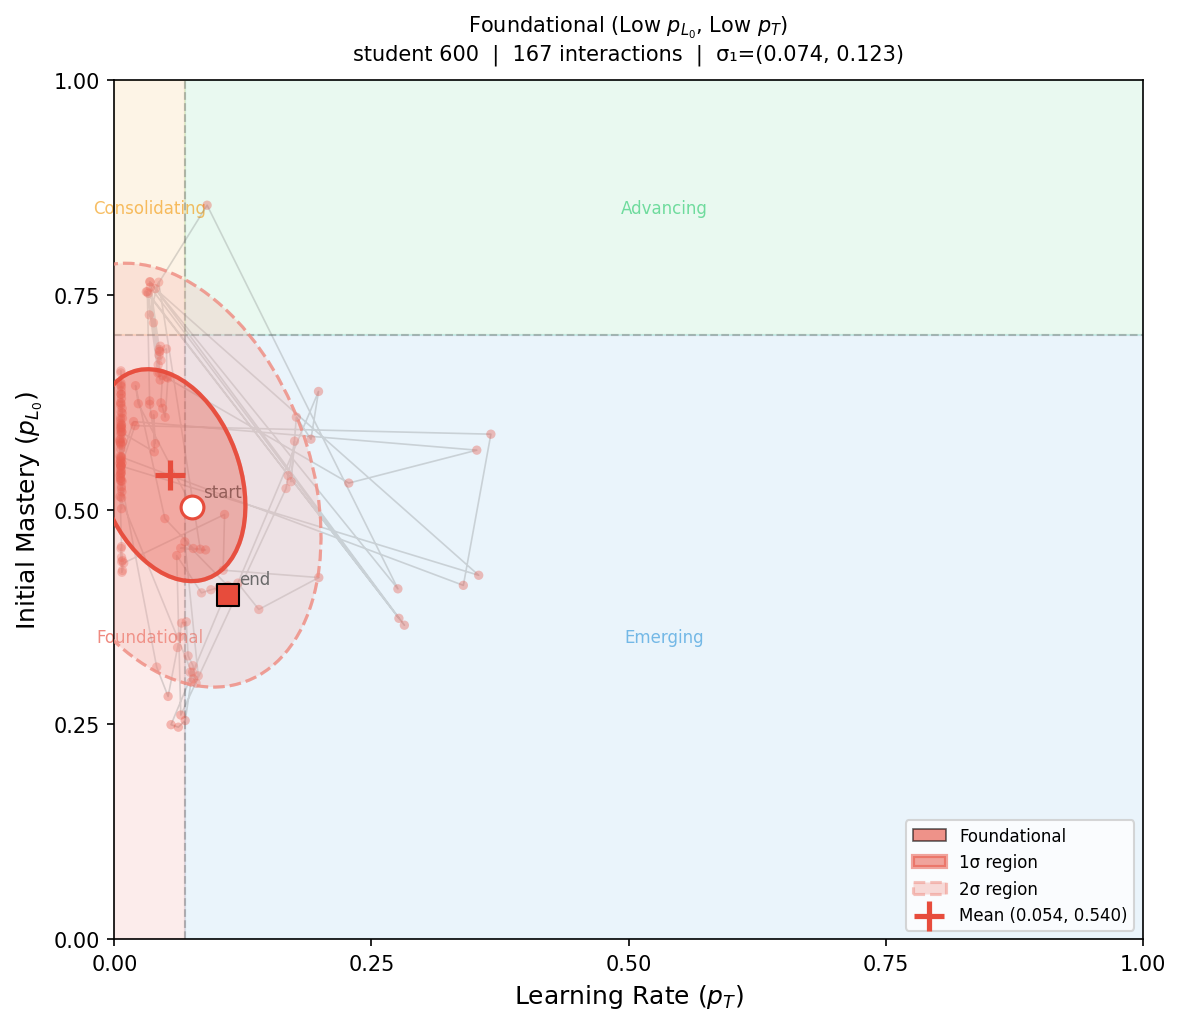
\includegraphics[width=\textwidth,height=0.30\textheight,keepaspectratio]{attractor_ellipse_foundational_893468.png}
  \caption{\textit{Foundational} ($p_{\text{L}_0}$, $p_{\text{T}}$).}
\end{subfigure}
\hfill
\begin{subfigure}[b]{0.48\textwidth}
  \centering
  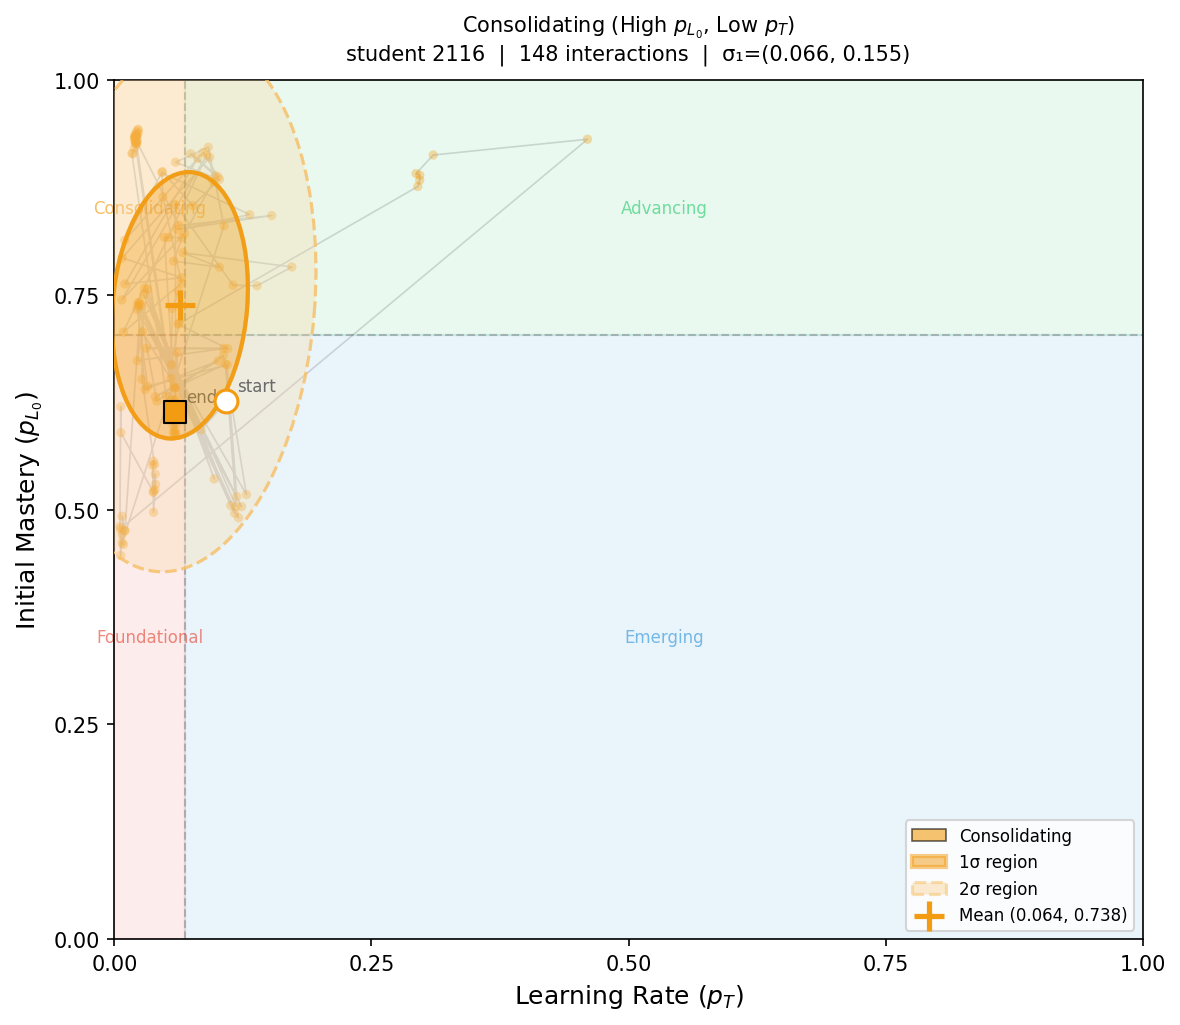
\includegraphics[width=\textwidth,height=0.30\textheight,keepaspectratio]{attractor_ellipse_consolidating_893468.png}
  \caption{\textit{Consolidating} ($p_{\text{L}_0}$, $p_{\text{T}}$).}
\end{subfigure}

\begin{subfigure}[b]{0.48\textwidth}
  \centering
  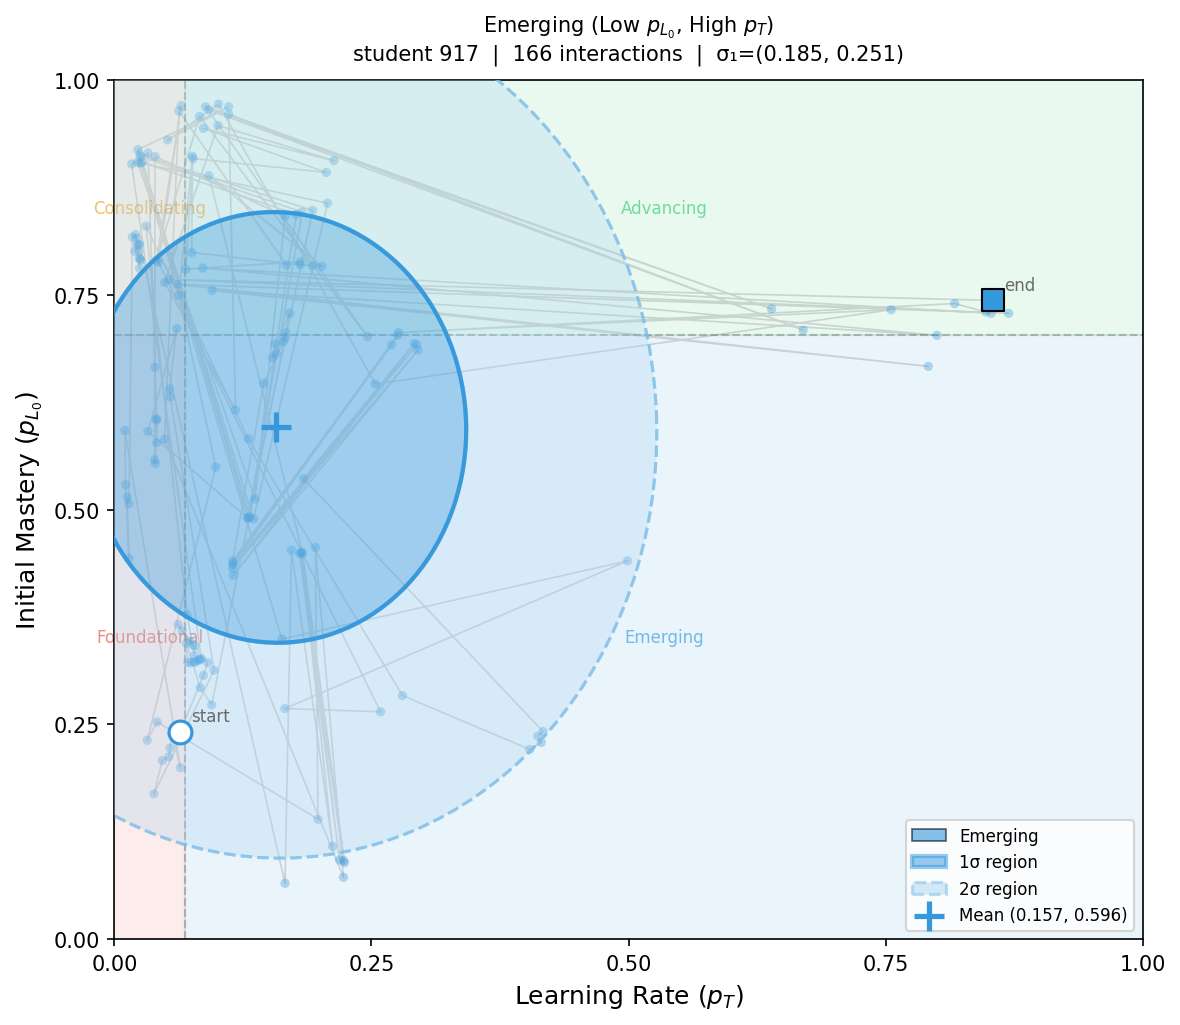
\includegraphics[width=\textwidth,height=0.30\textheight,keepaspectratio]{attractor_ellipse_emerging_893468.png}
  \caption{\textit{Emerging} ($p_{\text{L}_0}$, $p_{\text{T}}$).}
\end{subfigure}
\hfill
\begin{subfigure}[b]{0.48\textwidth}
  \centering
  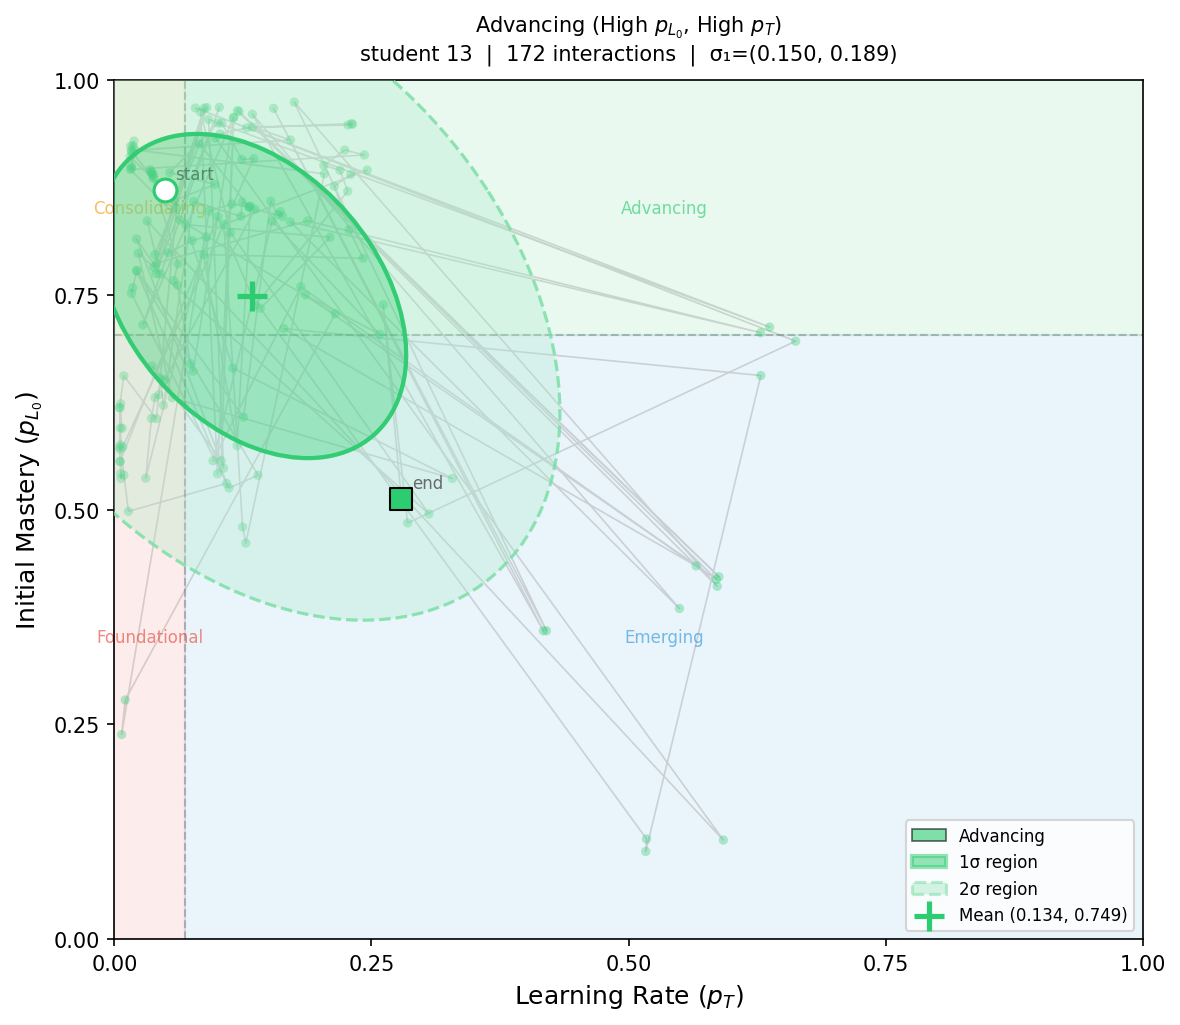
\includegraphics[width=\textwidth,height=0.30\textheight,keepaspectratio]{attractor_ellipse_advancing_893468.png}
  \caption{\textit{Advancing} ($p_{\text{L}_0}$, $p_{\text{T}}$).}
\end{subfigure}
\end{figure}

\subsection{Characteristics of the Four Learning Situations}

We estimated the grounded parameters associated with the learning trajectory of each student in the AS2009 dataset and used them to characterise student learning across the four learning situations. To investigate the characteristic dynamics of these situations, we selected a representative student for each quadrant who balances proximity to the quadrant centroid with interaction volume (weighted equally). 

Figure~\ref{fig_orbits} visualises their parameter orbits using covariance ellipses, which represent the temporal variation and density of the $(p_{\text{L}_0}, p_{\text{T}})$ estimates across each student's full interaction sequence. This longitudinal view makes explicit that a student's situation is not a static category frozen at enrolment, but a rolling summary of their evolving learning tendency as new interactions arrive. The ellipses in Figure~\ref{fig_orbits} specifically show:
\begin{itemize}
  \item \textit{Foundational} (low $p_{\text{L}_0}$, low $p_{\text{T}}$): the ellipse is compact and centred at low mastery and low learning rate, indicating limited contextual variation. Across interactions, the grounded estimates consistently assign this student low prior knowledge and a slow consolidation rate, reflecting a stable state of low mastery.
  \item \textit{Emerging} (low $p_{\text{L}_0}$, high $p_{\text{T}}$): the ellipse is the most spatially extended of all four situations, oriented along both the mastery and learning-rate axes. This broad orbit reflects a situation where parameters vary substantially across skills and contexts, indicating high growth potential.
  \item \textit{Consolidating} (high $p_{\text{L}_0}$, low $p_{\text{T}}$): the ellipse is compact and located at high mastery and low learning rate. The small spread indicates a stable region of the parameter space where prior knowledge is high but the per-interaction learning rate has converged toward zero.
  \item \textit{Advancing} (high $p_{\text{L}_0}$, high $p_{\text{T}}$): the ellipse is moderately extended and centred at high values for both mastery and learning rate. The spread confirms that this high-mastery situation is robust across different contexts and interactions.
\end{itemize}

\subsection{Dynamics of Learning Situation Trajectories}

While the orbit ellipses in Figure~\ref{fig_orbits} confirm that student learning situations are dynamic rather than static, they do not preserve the temporal sequence or direction of these changes. To capture this temporal evolution, we employ \textit{learning situation trajectories} that trace a student's movement through the $(p_{\text{T}}, p_{\text{L}_0})$ plane over time. These trajectories allow educators to observe whether a student's parameter pair is converging to a stable attractor, exhibiting rhythmic oscillations, or undergoing a transformative shift toward a different learning situation. By interpreting the length and orientation of trajectory segments, instructional designers can differentiate between students who are stagnating, those making steady progress, and those requiring immediate intervention, thus providing a transparent and actionable diagnostic tool for human-in-the-loop oversight. 

Figure~\ref{fig_trajectories} shows the trajectory plot for the representative student of each learning situation on the AS2009 dataset. Each panel traces consecutive sampled interactions in the $(p_{\text{T}}, p_{\text{L}_0})$ plane. The representative for each quadrant is the student who maximises a composite score balancing proximity to the quadrant centroid and number of interactions (equal weights). A candidate point is sampled every 5 interactions and retained only when its Euclidean distance from the last plotted point exceeds $\delta_{\min}\approx 0.3$; otherwise it is absorbed into the preceding point, whose marker area grows proportionally to encode dwell time. The $p_{\text{T}}$ axis is capped at 0.5 to exclude a small fraction of high-rate outlier interactions ($<$6\%). The first and last directional arrows are rendered in a darker tone to temporally anchor the trajectory; all intermediate arrows are in light grey. Coloured background regions delimit the four learning situations; a point may cross boundaries, indicating a genuine shift over time.

The four trajectories are qualitatively distinct in ways that are directly instructionally informative.

\begin{itemize}
\item The \textit{foundational} student (120 interactions, 8 plotted points) remains anchored in the lower-left quadrant throughout, with transient fluctuations that consistently return to low mastery and low learning rate, indicating that current instructional conditions are insufficient to drive durable progress.
\item The \textit{consolidating} student (148 interactions, 3 plotted points) yields the most compact trajectory of all four: the large marker at the terminal point (interaction 25) encodes the 123 subsequent interactions that produced no displacement exceeding $\delta_{\min}$, making the prolonged absence of movement the primary visible signal of stagnation rather than the parameter values themselves.
\item The \textit{emerging} student (156 interactions, 15 plotted points, after excluding a small fraction of high-rate outliers with $p_T > 0.5$) produces the most spatially extended orbit, crossing all four quadrants; both $p_{L_0}$ and $p_T$ oscillate with large steps across a wide portion of the visible range, making parameter variability the defining feature of this trajectory rather than convergence to a stable attractor.
\item The \textit{advancing} student (168 interactions, 4 plotted points) shows consistently high prior mastery combined with above-median learning rates throughout; the large marker at the final plotted point encodes the remaining interactions, confirming that the parameter pair stays in the upper-right region for the bulk of the trajectory. 
\end{itemize}

By reading these trajectories, educators gain theory-grounded evidence of whether a student is disengaging (decreasing $p_{\text{T}}$), stagnating (stable high $p_{\text{L}_0}$, falling $p_{\text{T}}$), or actively learning (increasing parameters, boundary crossings); evidence that supports intentional instructional decision-making and satisfies the accountability requirements for high-risk educational AI.


\begin{figure}[!htb]
\caption{\textit{Learning situation trajectories.} Each plot traces the evolution of the grounded parameters pair for the representative student of one learning situation in the AS2009 dataset. Marker area encodes dwell time (interactions absorbed between two plotted points). The first and last arrows are rendered in a darker tone; all intermediate arrows are in light grey. The $p_{\text{T}}$ axis is capped at 0.5. Coloured background regions delimit the four learning situations.}
\label{fig_trajectories}
\centering
\begin{subfigure}[b]{0.48\textwidth}
  \centering
  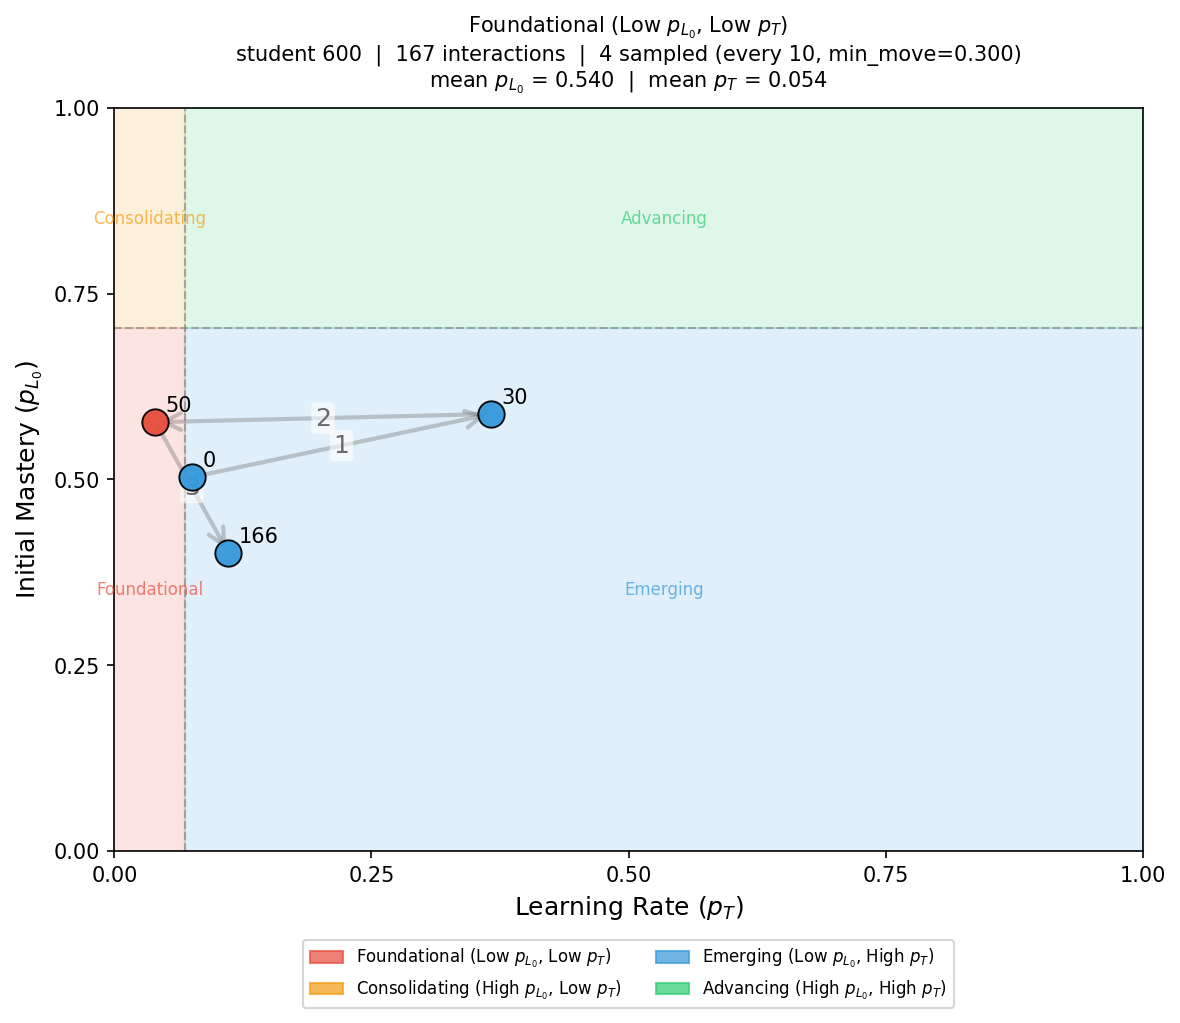
\includegraphics[width=\textwidth,height=0.30\textheight,keepaspectratio]{roster_2d_foundational_893468.png}
  \caption{\textit{Foundational} (low $p_{\text{L}_0}$, low $p_{\text{T}}$).}
\end{subfigure}
\hfill
\begin{subfigure}[b]{0.48\textwidth}
  \centering
  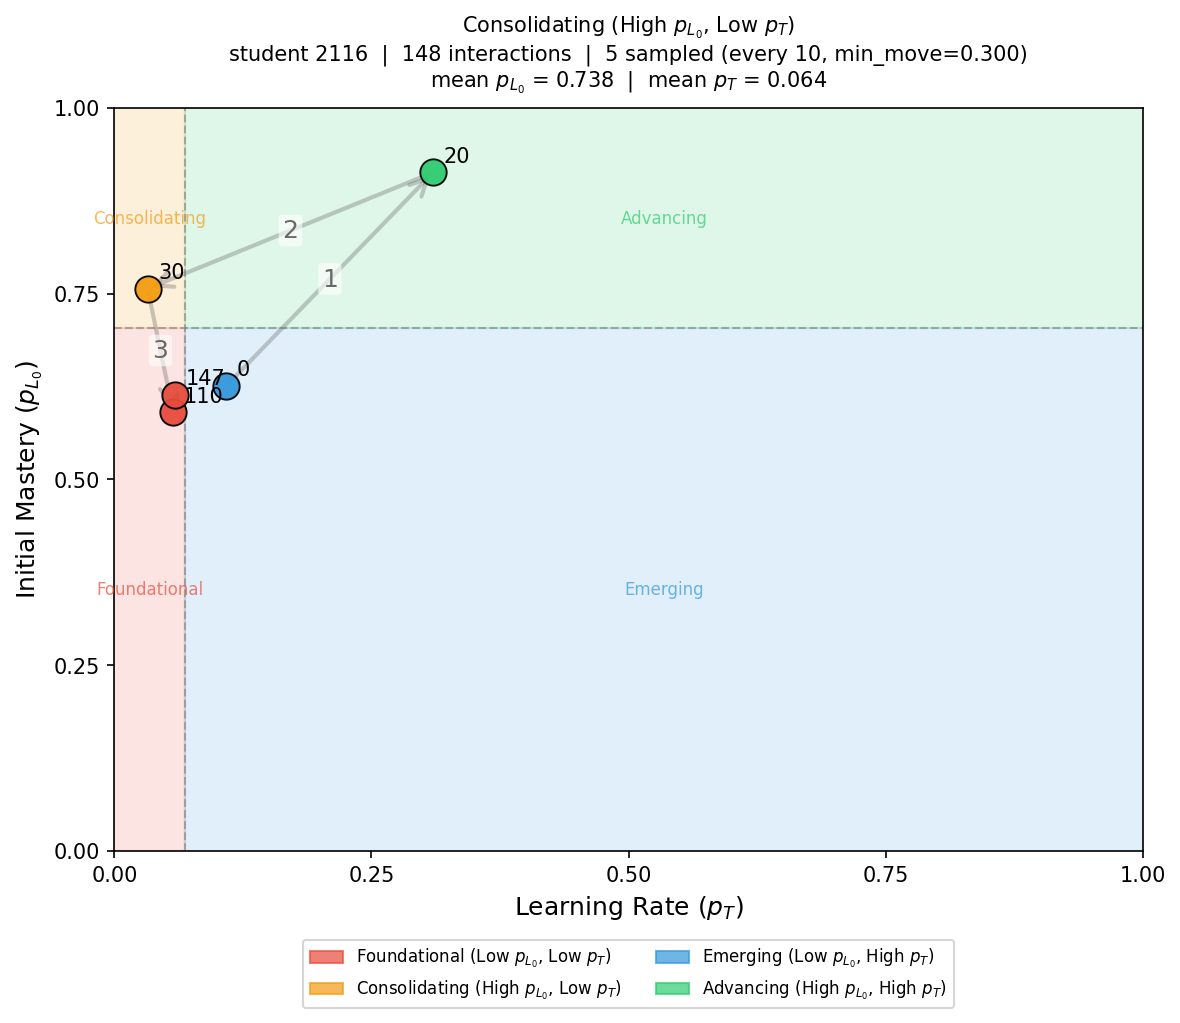
\includegraphics[width=\textwidth,height=0.30\textheight,keepaspectratio]{roster_2d_consolidating_893468.png}
  \caption{\textit{Consolidating} (high $p_{\text{L}_0}$, low $p_{\text{T}}$).}
\end{subfigure}

\begin{subfigure}[b]{0.48\textwidth}
  \centering
  
\includegraphics[width=\textwidth,height=0.30\textheight,keepaspectratio]{roster_2d_emerging_893468.png}
  \caption{\textit{Emerging} (low $p_{\text{L}_0}$, high $p_{\text{T}}$).}
\end{subfigure}
\hfill
\begin{subfigure}[b]{0.48\textwidth}
  \centering
  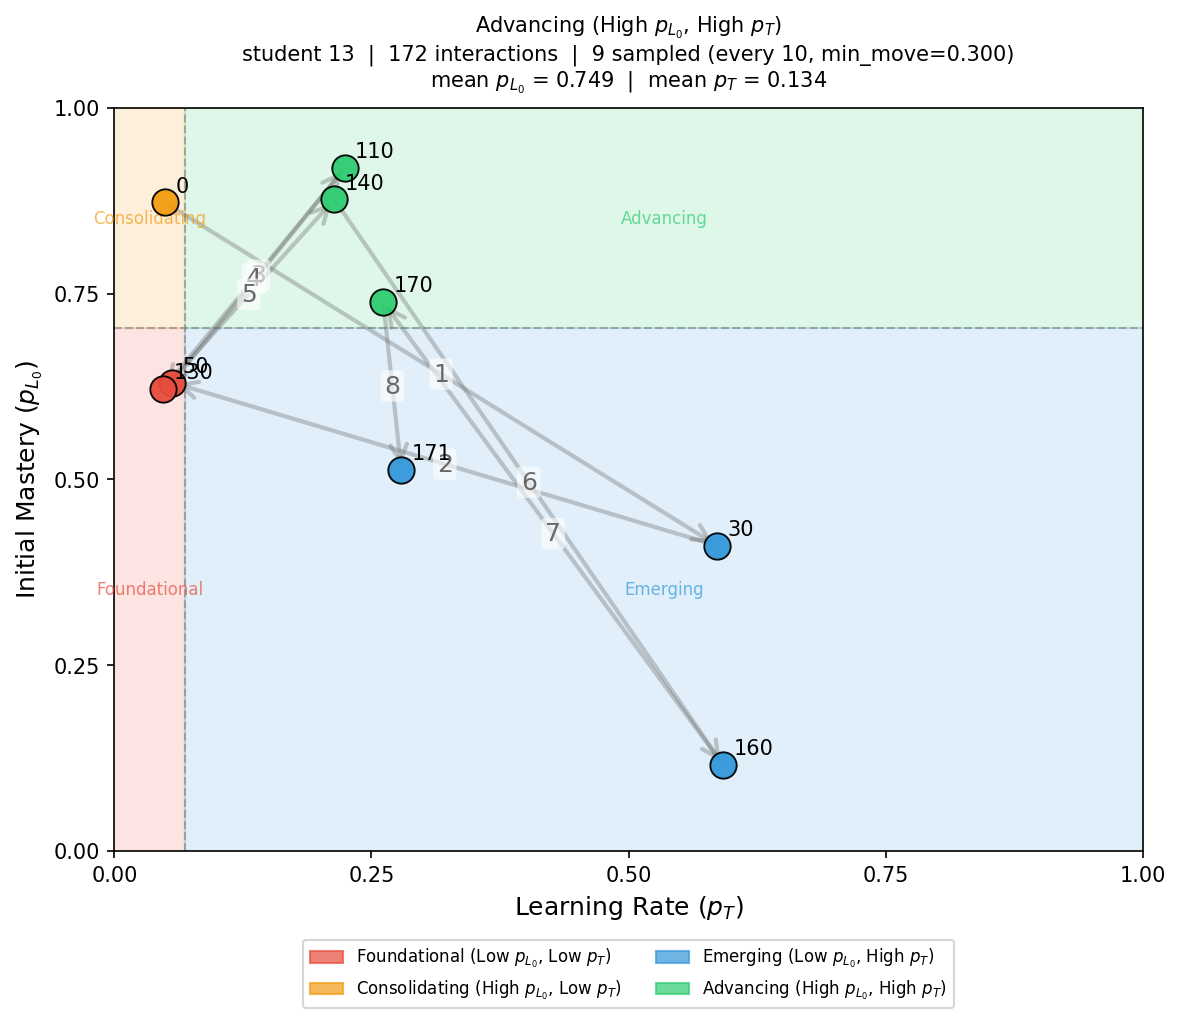
\includegraphics[width=\textwidth,height=0.30\textheight,keepaspectratio]{roster_2d_advancing_893468.png}
  \caption{\textit{Advancing} (high $p_{\text{L}_0}$, high $p_{\text{T}}$).}
\end{subfigure}
\end{figure}

\begin{figure}[!htb]
  \centering
  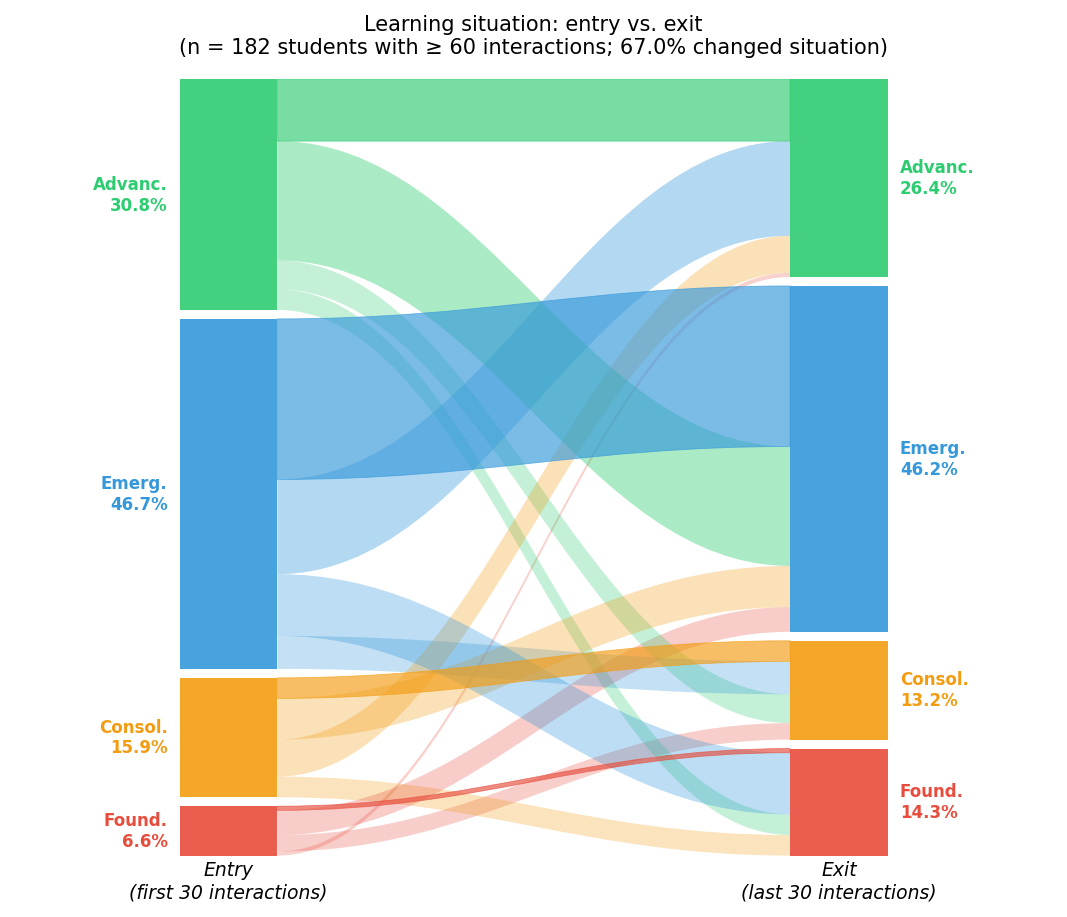
\includegraphics[width=0.8\textwidth,keepaspectratio]{situation_alluvial_893468.png}
  \caption{Learning situation at session entry (first 30 interactions) versus session exit (last 30 interactions) for $n = 182$ students with at least 60 interactions. Ribbon width is proportional to the fraction of students. Ribbons are coloured by entry situation; crossing ribbons indicate a change of learning situation over the course of the session. 67.0\% of students were assigned a different learning situation at the end of their session.}
  \label{fig_transitions}
\end{figure}

\subsection{Dynamic Nature of Learning Situations}

Figure~\ref{fig_transitions} illustrates the dynamic nature of these assignments. Of the 182 AS2009 students with at least 60 interactions, 67\% were assigned a different learning situation at session exit (last 30 interactions) versus session entry (first 30 interactions). This high transition rate confirms that the augmented model captures genuine learning dynamics rather than stable individual traits, and that situation-based routing responds to the student's observed trajectory rather than to a fixed initial categorisation.

\section{Conclusions}

This paper contributed an augmented student model for Intelligent Tutoring Systems that operationalises the principle of shaping technology with learning theory. This design marks a fundamental shift from purely accuracy-driven student modelling to a more mindful approach grounded in pedagogically sound principles. By augmenting the user model with theory-grounded parameter estimates, our system supports both transparent diagnostics, through the detection of distinct learning situations, and purposeful instructional actions through evidence-based strategies. This approach directly benefits students by enabling dynamic, personalised adaptation to their evolving needs, while simultaneously empowering educators through an interpretable architecture that guarantees human agency and accountability in automated educational environments.

%
\begin{credits}
\subsubsection{\ackname}
This research received no external funding.

\subsubsection{\discintname}
The authors have no competing interests to declare that are relevant to the content of this article.
\end{credits}

%
\begin{thebibliography}{99}
\providecommand{\url}[1]{\texttt{#1}}
\providecommand{\urlprefix}{URL }
\providecommand{\doi}[1]{https://doi.org/#1}

\bibitem{itssleeman82}
Auguste, D.: Intelligent tutoring systems: {D}. {S}leeman and {J}.{S}. {B}rown,
  (academic press, new york, 1982); 345 pages, \$39.50. Artificial Intelligence
   \textbf{26}(2),  233--238 (1985). \doi{10.1016/0004-3702(85)90033-5}

\bibitem{corbett1994knowledge}
Corbett, A.T., Anderson, J.R.: Knowledge tracing: Modeling the acquisition of
  procedural knowledge. User modeling and user-adapted interaction
  \textbf{4}(4),  253--278 (1994)

\bibitem{piech2015deep}
Piech, C., Bassen, J., Huang, J., Ganguli, S., Sahami, M., Guibas, L.J.,
  Sohl-Dickstein, J.: Deep knowledge tracing. Advances in neural information
  processing systems  \textbf{28} (2015)

\bibitem{ghosh2020context}
Ghosh, A., Heffernan, N., Lan, A.S.: Context-aware attentive knowledge tracing.
  In: 26th ACM SIGKDD international conference on knowledge discovery \& data
  mining. pp. 2330--2339 (2020)

\bibitem{labra2026theory}
Labra, C., Santos, O.C.: {Theory-Based Interpretability in Deep Knowledge
  Tracing via Grounded Transformers}. Applied Sciences  \textbf{16}(7), ~3138
  (2026)

\bibitem{yudelson2013individualized}
Yudelson, M.V., Koedinger, K.R., Gordon, G.J.: Individualized {Bayesian}
  knowledge tracing models. In: International conference on artificial
  intelligence in education. pp. 171--180. Springer (2013)

\bibitem{abdelrahman2023knowledge}
Abdelrahman, G., Wang, Q., Nunes, B.: Knowledge tracing: A survey. ACM
  Computing Surveys  \textbf{55}(11),  1--37 (2023)

\bibitem{rudin2019stop}
Rudin, C.: Stop explaining black box machine learning models for high stakes
  decisions and use interpretable models instead. Nature machine intelligence
  \textbf{1}(5),  206--215 (2019)

\bibitem{nkambou2010advances}
Nkambou, R., Mizoguchi, R., Bourdeau, J.: Advances in intelligent tutoring
  systems (2010)

\bibitem{Holmes2022504}
Holmes, W., Porayska-Pomsta, K., Holstein, K., Sutherland, E., Baker, T., Shum,
  S.B., Santos, O.C., Rodrigo, M.T., Cukurova, M., Bittencourt, I.I.,
  Koedinger, K.R.: Ethics of ai in education: Towards a community-wide
  framework. International Journal of Artificial Intelligence in Education
  \textbf{32}(3),  504--526 (2022). \doi{10.1007/s40593-021-00239-1}

\bibitem{feng2009addressing}
Feng, M., Heffernan, N., Koedinger, K.: Addressing the assessment challenge
  with an online system that tutors as it assesses. User modeling and
  user-adapted interaction  \textbf{19}(3),  243--266 (2009)

\end{thebibliography}

\end{document}
